% ICMC 2006 paper template for Latex2e.

% Points to note:
%    Please use \paragraph instead of \subsubsection -- see discussion below.
%    See comments in the References section on how to do citations.

\documentclass[10pt,letterpaper]{article}
\usepackage{graphicx}
\usepackage{subfigure}
\usepackage{fullpage}
\usepackage{times}
\usepackage{chicago}                    % for "(Author, year)" cite style.
\usepackage{indentfirst}                % indent para after headings.
% \usepackage{url}                      % (handy if you reference a URL.)

\setlength{\oddsidemargin}{-0.25in}     % Latex has one-inch "driver margin"
% \setlength{\evensidemargin}{-0.25in}  % (shouldn't be necessary)
\setlength{\textwidth}{7in}             % 8.5 - 2*0.75 

\setlength{\columnsep}{0.25in}
\setlength{\parindent}{0.2in}

\raggedbottom                           % better than inter-para spaces, I say.


\begin{document}

\twocolumn

\title{\textbf{Musical Tapestry: Re-composing Natural Sounds}}
\author{
Ananya Misra, Perry R. Cook$^{\dag}$, Ge Wang\\
Department of Computer Science ($^{\dag}$also Music), Princeton University \\
amisra/prc/gewang@cs.princeton.edu\\
}
\date{}     % no date
\maketitle

\pagestyle{empty}          % no page numbers.
\thispagestyle{empty}      % yes, that includes not on the first page, either.

% do abstract by hand -- \begin{abstract} wouldn't conform to the guidelines.

\begin{center}
\large{\textbf{Abstract}}
\end{center}
% there's this annoying little indent here I can't properly eliminate, so...
\hspace*{-0.1in}                       % hackily cancel it out.
\noindent
\textit{
A system to aid composition with analysis and resynthesis 
of natural sounds is described.  Sinusoidal analysis is 
used to isolate and extract deterministic sounds, and 
transients are also isolated/extracted, leaving the 
stochastic background sound which is parameterized 
by wavelet tree analysis.   All of these components 
become templates for the synthesis phase, which is 
controlled 1) by placing templates on timelines,
2) by real-time manipulation of parameter sliders,
and 3) via a scripting language based on the ChucK
language.  The result is a flexible ``workbench''
for doing modern day musique concr\`{e}te or acousmatic
composition, sound design, and other sonic sculpting
tasks.
}

\begin{figure*}[tbh!]
\centering
    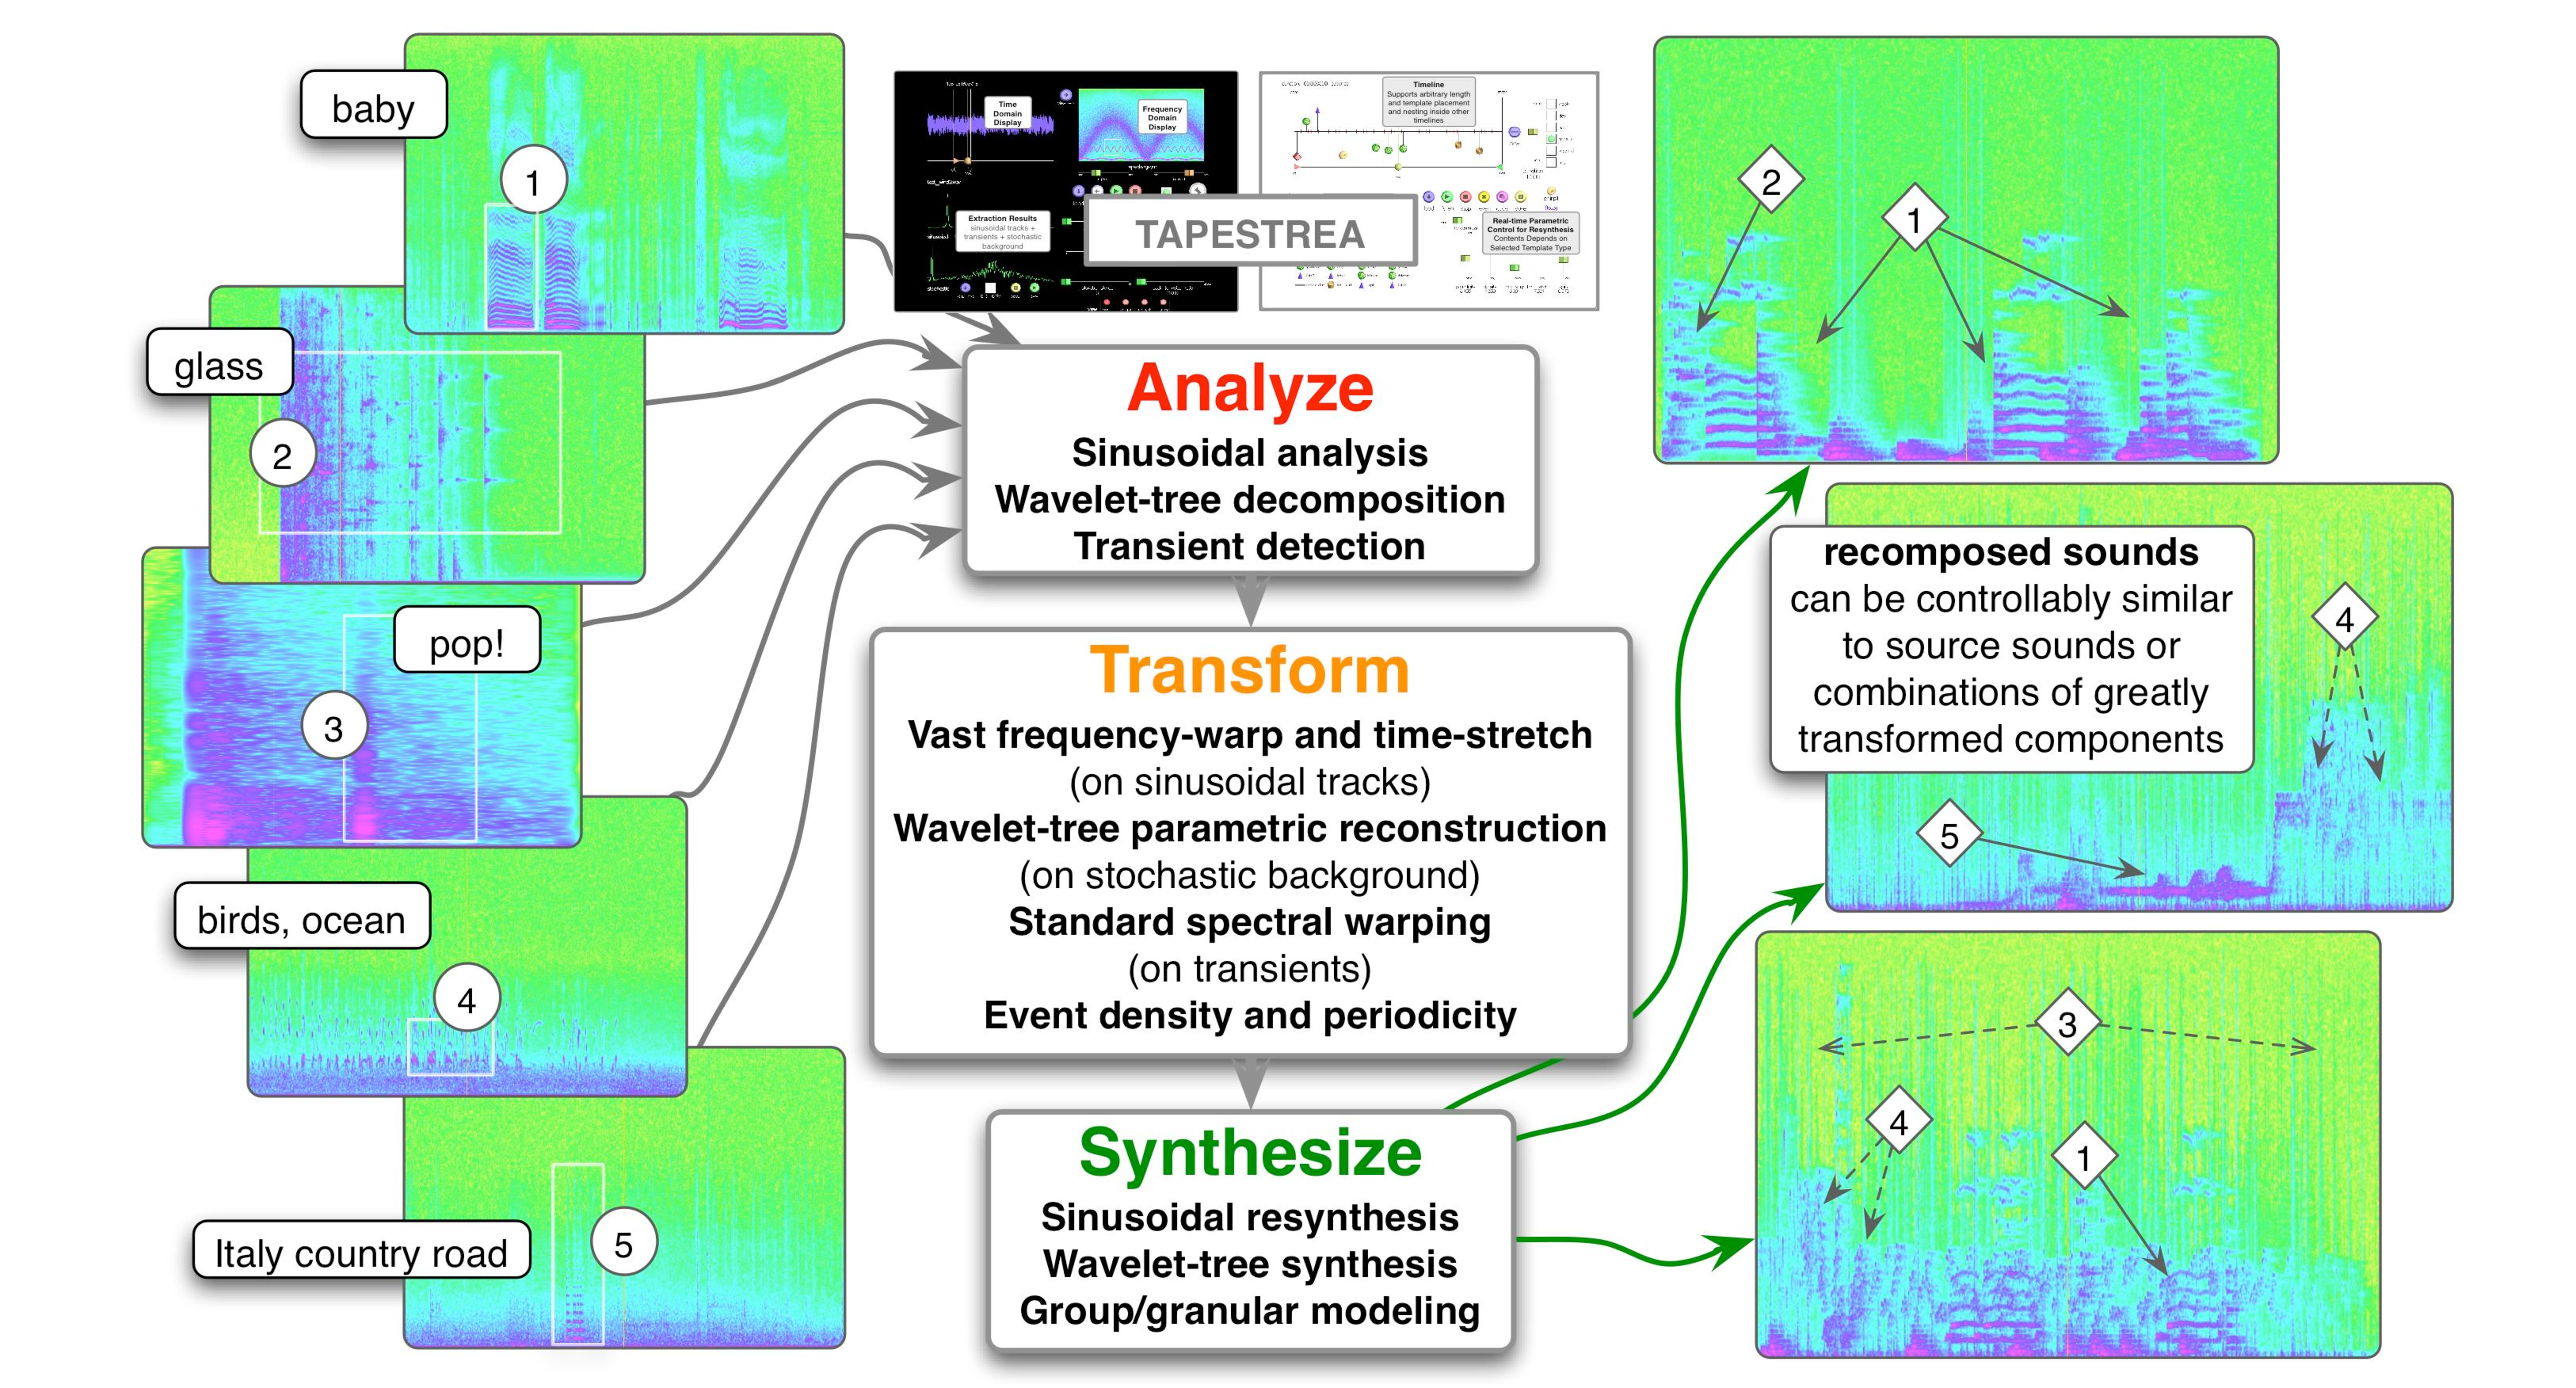
\includegraphics[width=.95\textwidth]{teaser.pdf}
    \caption{\textbf{Designing musical tapestries}.  User-selected regions of input sounds (left) are 
    analyzed into reusable templates, which are separately transformed, and resynthesized.
    Numbered diamonds (right) correspond to instances of sound components (circled, left).
    The framework allows flexible control at every stage in the proces.} 
    \label{fig:teaser}
\end{figure*}

\section{Introduction}

In the 1940s and 50s, Pierre Schaeffer developed musique
concr\`{e}te~\cite{Schaeffer50,Schaeffer52}.  Unlike traditional music,
musique concr\`ete starts with existing or concrete recorded sounds,
which are organized into abstract musical structures. The existing
recordings often include natural and industrial sounds that are not
conventionally musical, but can be manipulated to make music, either by
editing magnetic tape or now more commonly through digital sampling.
Typical manipulations include cutting, copying, reversing, looping and
changing the speed of recorded segments.

Today, several other forms of electronic/electroacoustic music also
involve manipulating a set of recorded sounds. Acousmatic
music~\cite{Dhomont95}, for instance, evolved from musique concr\`ete
and refers to compositions designed for environments that emphasize the
sound itself rather than the performance-oriented aspects of the piece.

The acoustic ecology~\cite{Schafer77} movement gave rise to soundscape
composition~\cite{Truax96,Truax02} or the creation of realistic
soundscapes from recorded environmental audio. One of the key features
of soundscape composition, according to Truax, is that ``most pieces can
be placed on a continuum between what might be called `found sound' and
`abstracted' approaches.'' However, while ``contemporary signal processing
techniques can easily render such sounds unrecognizable and completely
abstract,'' a soundscape composition piece remains recognizable even at
the abstract end of the continuum.

Sound designers for movies, theater and art often have a related goal of
starting with real world sounds and creating emotionally evocative sound
scenes, which are still real, yet transformed and transformative.
Classic examples include mixing a transformed lion's roar with other
sounds to accompany the wave sounds in \textit{The Perfect Storm}, and
incorporating a helicopter theme into the sound design for \textit{Black
Hawk Down}~\cite{Rudy04} These sound designers are ``sound sculptors''
as well, but transform sounds to enhance or create a sense of reality,
rather than for purely musical purposes.

Artists from all of the above backgrounds share the process
of manipulating recordings, but aim to achieve different
effects. We present a single framework for starting with
recordings and producing sounds that can lie anywhere on a
`found' to `unrecognizable' continuum. `Found' sounds can
be modified in subtle ways or extended indefinitely, while
moving towards the `unrecognizable' end of the spectrum unleashes
a range of manipulations beyond time-domain techniques.
In fact, the same set of techniques apply throughout
the continuum, differing only in how they are used. We call
this framework TAPESTREA: Techniques and Paradigms for
Expressive Synthesis, Transformation and Rendering of Environmental
Audio.

TAPESTREA integrates sinusoidal analysis, stochastic background modeling, transient detection, and a new class of user interface that lends itself to any composition that originates in recorded environmental audio. This envelopes a novel form of musique concr\`ete that extends to manipulations in the frequency as well as time domain. Advantages of the TAPESTREA approach include: 

1. Existing composition techniques based on recordings of natural sounds are often time-domain-centric. Even with more spectrally oriented tools such as the phase vocoder, the source is a segment cut ``out of time.'' While supporting this notion and practice, TAPESTREA also leverages the power of sinusoidal analysis and re-synthesis to allow extraction, transformation, and re-synthesis in the frequency domain. The sound sculptor is able to select a region in both time and frequency, essentially specifying, ``Give me \textit{this} part of \textit{that} sound,'' to extract a transformable and reusable \textit{sound template}.

2. TAPESTREA distinguishes between three fundamental types of sound components, based on the modeling techniques to which they are best suited. Deterministic (sinusoidal), transient, and stochastic background components are modeled separately, using methods to which they are most amenable, leading to a powerful range of transformations. 

3. To realize these ideas, TAPESTREA provides a new interface that allows the sound designer or composer to treat each component type and each phase of the sculpting process in an independent and parametrically controlled, yet overall cohesive manner. 

TAPESTREA manipulates recorded sounds in two phases. In the analysis
phase, the sound is separated into reusable components that map to
individual foreground events or background. In the synthesis phase,
these components are parametrically transformed, combined and
re-synthesized using time- and frequency-domain techniques that can be
controlled on multiple levels. While we highlight the synthesis methods
here, the analysis phase is also integral as it enables the
most flexible means for dealing with real-world sonic material.

\section{Related Work}

Related techniques used for musical composition include spectral modeling
synthesis~\cite{Serra89} and granular 
synthesis~\cite{Truax88,Truax90,Roads02}. Spectral modeling synthesis 
separates a sound into sinusoids and
noise, and was originally used for modeling instrument sounds. Granular
synthesis, in contrast, functions in the time-domain and involves
continuously controlling very brief sonic events or sound grains. TAPESTREA
employs aspects of both, using separation techniques on environmental sounds
and controlling the temporal placement of resulting events.

Another technique used in TAPESTREA is an extension of a wavelet tree
learning algorithm~\shortcite{Dubnov02} for sound texture synthesis. This
method performs a wavelet decomposition on a sound clip and uses machine
learning on the wavelet coefficients to generate similar non-repeating sound
texture. The algorithm works well for sounds that are mostly stochastic, but
can break extended pitched portions in objectionable ways. It can also be 
slow in its original form. TAPESTREA takes advantage of this technique by 
improving the speed of the algorithm, and only using it on the types of 
(non-deterministic) sound for which it works well.

\section{Analysis Phase}

\begin{figure}[h]
  \begin{center}
%    \framebox[7cm]{\rule[-5mm]{0cm}{5cm} }
    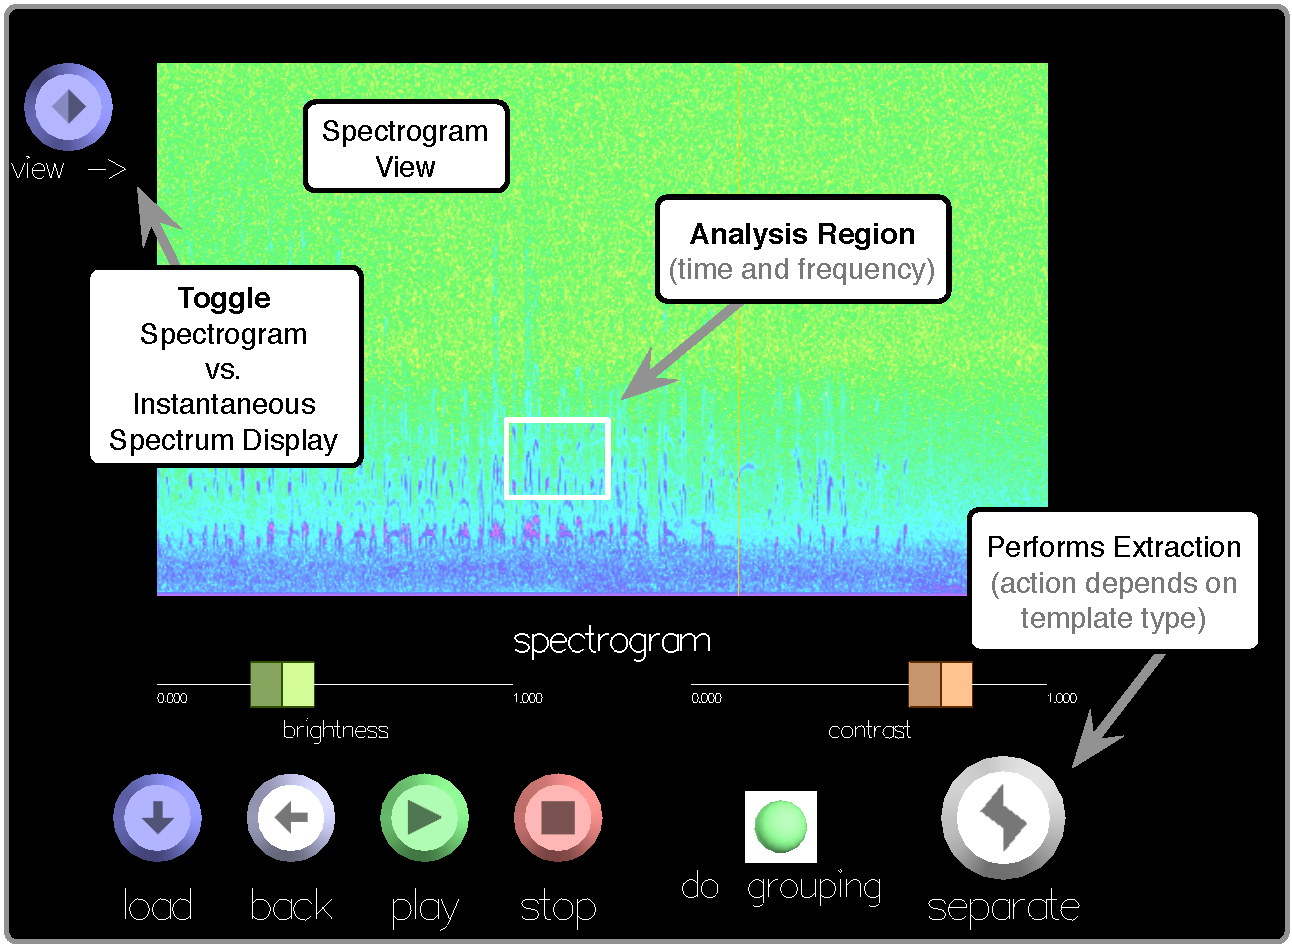
\includegraphics[width=.95\columnwidth]{ui_specgram.pdf}
    \caption{Spectrogram view in analysis face.} 
    \label{fig:ui_specgram}
  \end{center}
\end{figure}

TAPESTREA starts by separating a recording into \textit{deterministic
events} or the stable sinusoidal components of the
sound, \textit{transient events} or brief noisy bursts of energy, and the
remaining \textit{stochastic background} or din. This separation can
be parametrically controlled and takes place in the analysis
phase. 

The analysis interface is shown in the accompanying figures. A loaded sound is simultaneously displayed in the form of a form of a waveform and a spectrogram (Figure \ref{fig:ui_specgram}). The spectrogram display can also be toggled with a frame-by-frame spectrum view (Figure \ref{fig:ui_spectrum}). Selecting a rectangle on
the spectrogram, or selecting an analysis region on the waveform and the
frame-by-frame spectrum, limits the analysis to the associated time and
frequency ranges, facilitating the selection and extraction of
specific events. 

\begin{figure}[h]
  \begin{center}
%    \framebox[7cm]{\rule[-5mm]{0cm}{5cm} }
    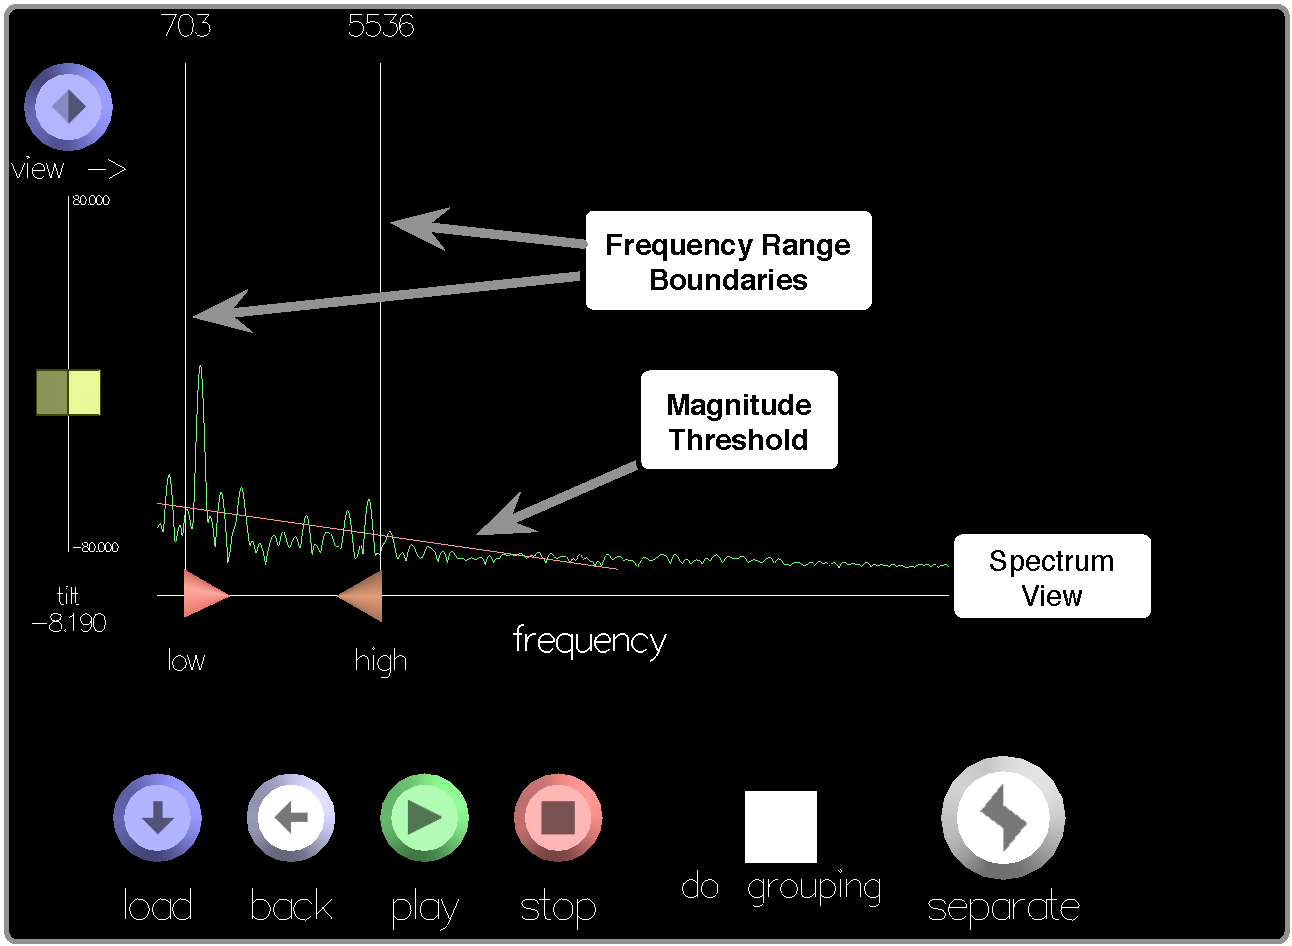
\includegraphics[width=.95\columnwidth]{ui_spectrum.pdf}
    \caption{Spectrum view in analysis face.} 
    \label{fig:ui_spectrum}
  \end{center}
\end{figure}

\textit{Deterministic events} are foreground events extracted by
sinusoidal modeling based on the spectral modeling
framework~\cite{Serra89}. Overlapping frames of the sound are
transformed into the frequency domain using the FFT. For each spectral
frame, the \textit{n} highest peaks above a specified magnitude threshold (Figure \ref{fig:ui_spectrum}) are
recorded, where \textit{n} can range from 1 to 50. These peaks can also be loaded
from a preprocessed file. The highest peaks from every frame are then
matched across frames by frequency, subject to a controllable ``frequency
sensitivity'' threshold, to form sinusoidal tracks. Tracks can be ``mute''
or below the magnitude threshold for a specified maximum number of
frames, or can be discarded if they fail to satisfy a minimum track
length requirement (Figure \ref{fig:ui_sines}). 

\begin{figure}[h]
  \begin{center}
%    \framebox[7cm]{\rule[-5mm]{0cm}{5cm} }
    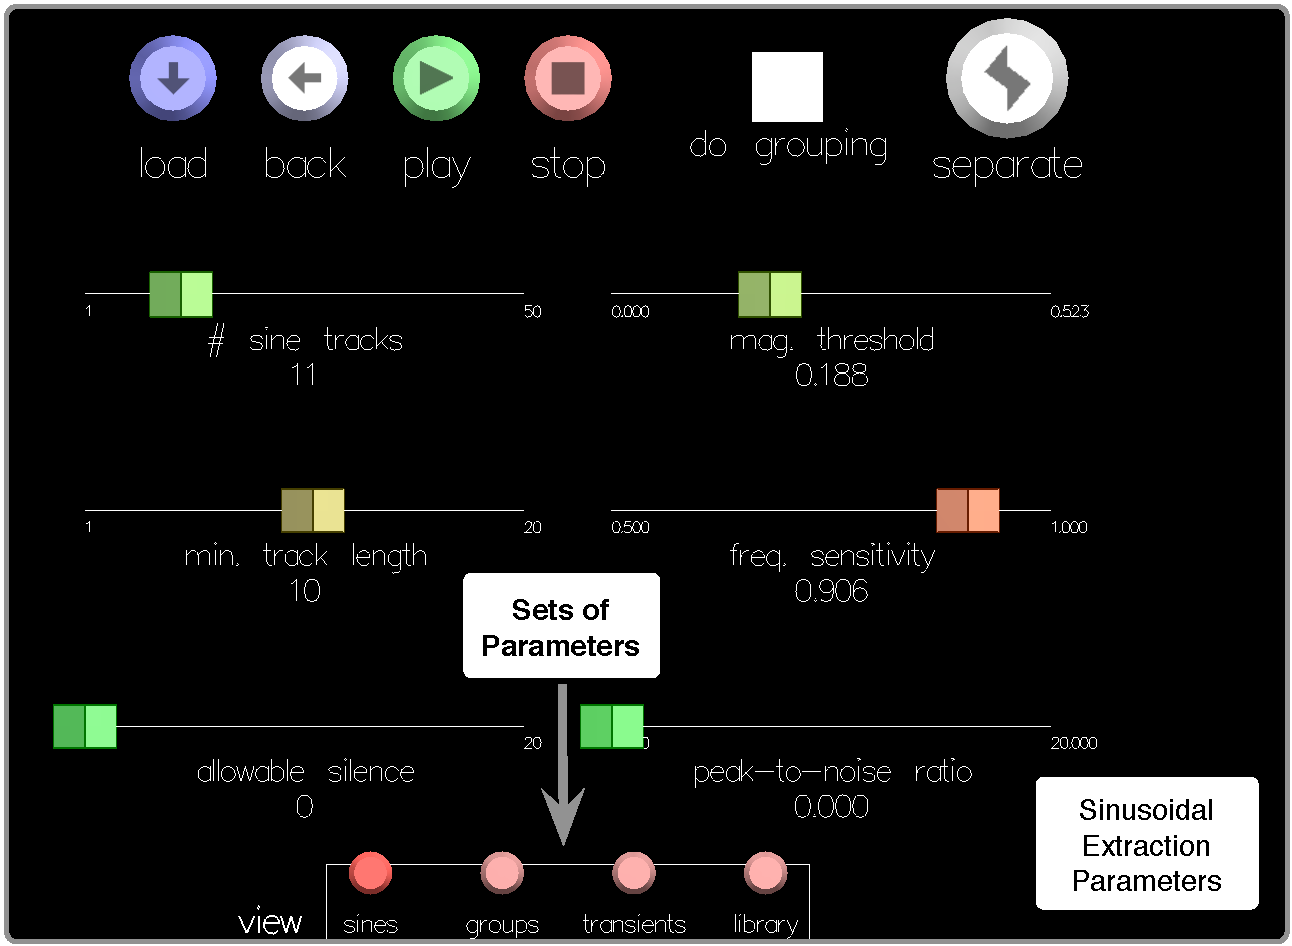
\includegraphics[width=.95\columnwidth]{ui_sliders1.pdf}
%    \subfigure[]{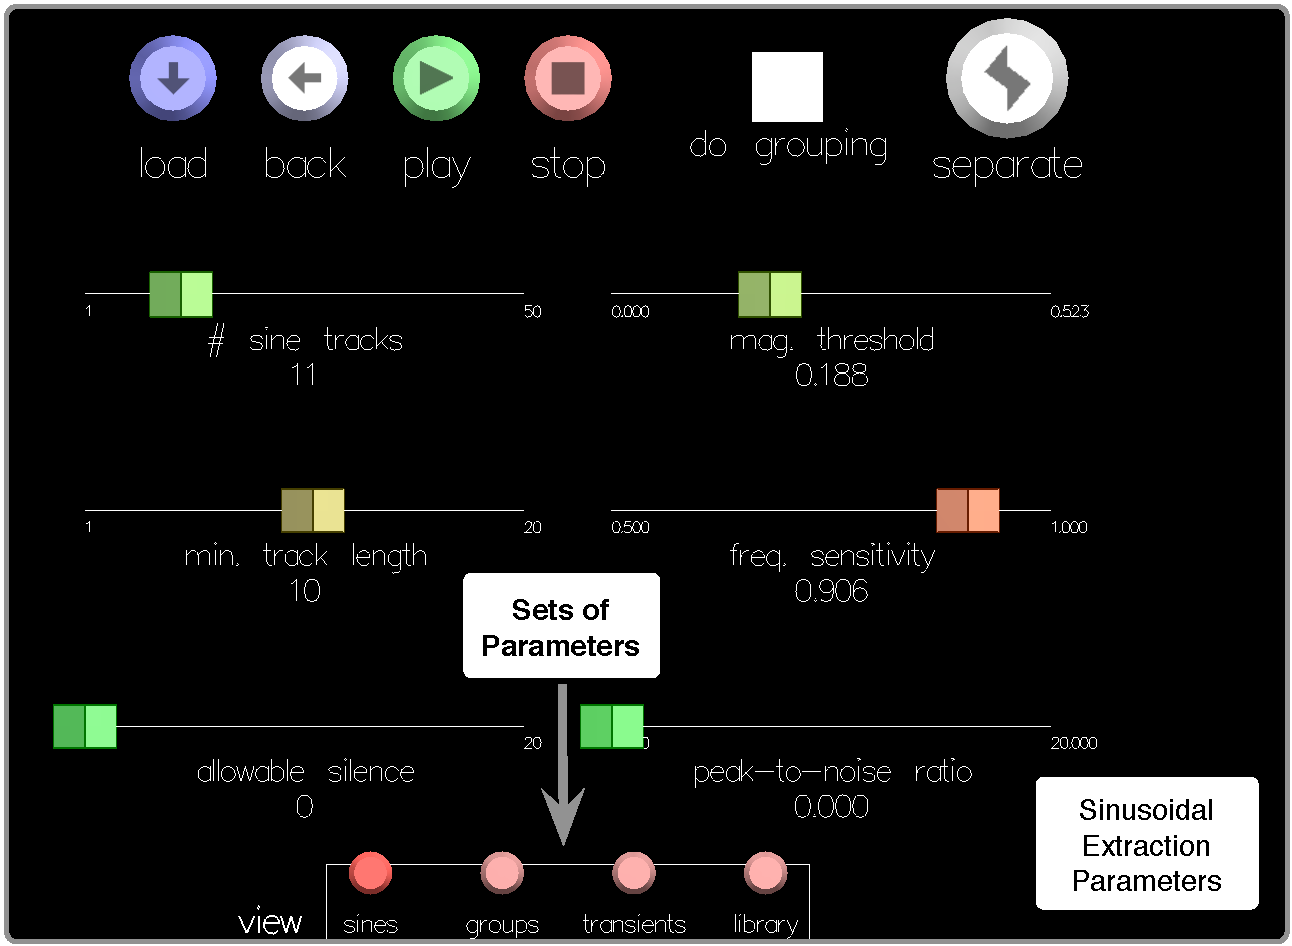
\includegraphics[width=.48\columnwidth]{ui_sliders1.pdf}}
%    \subfigure[]{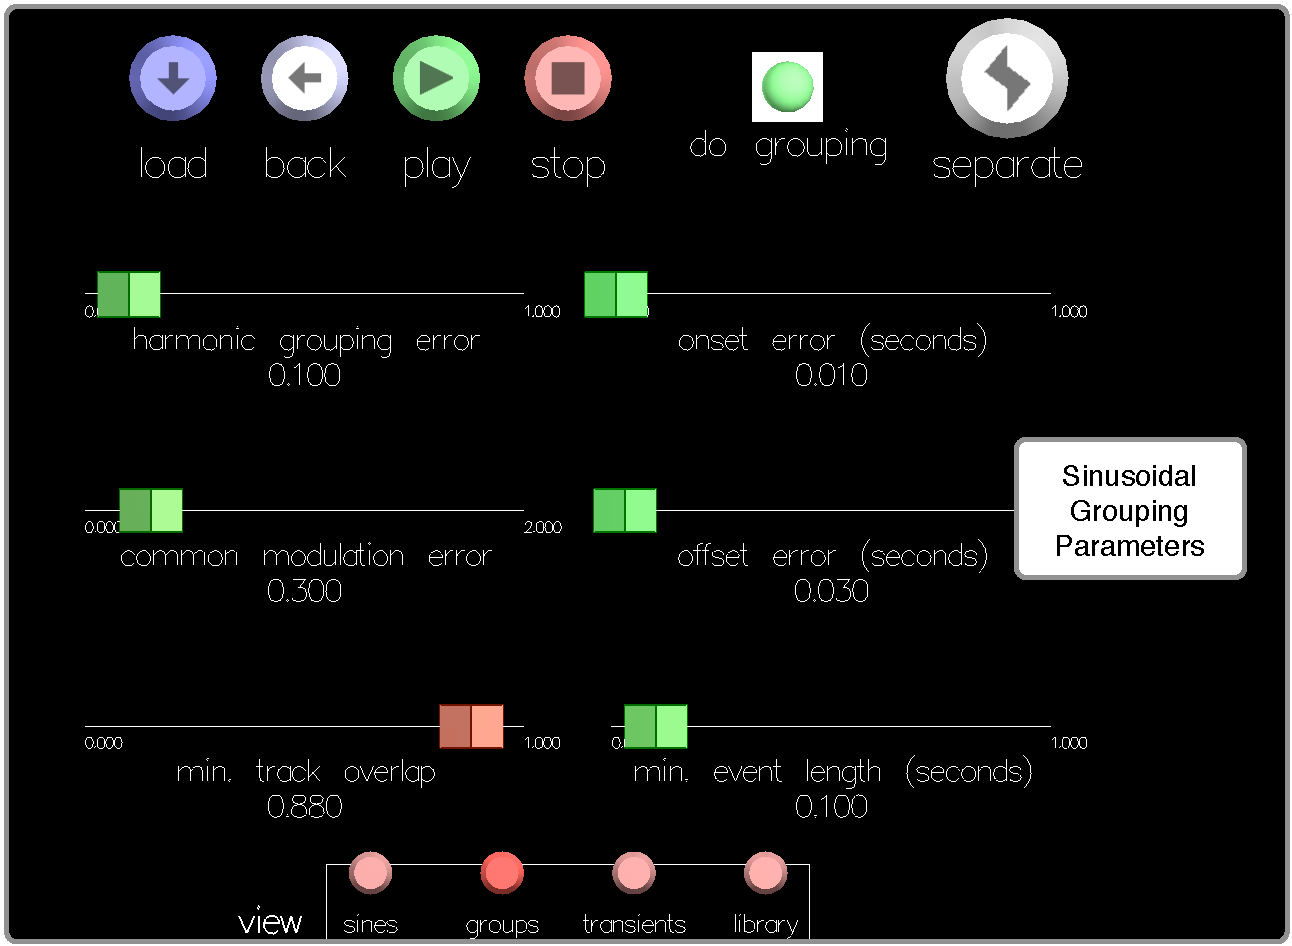
\includegraphics[width=.48\columnwidth]{ui_sliders2.pdf}}
%    \subfigure[]{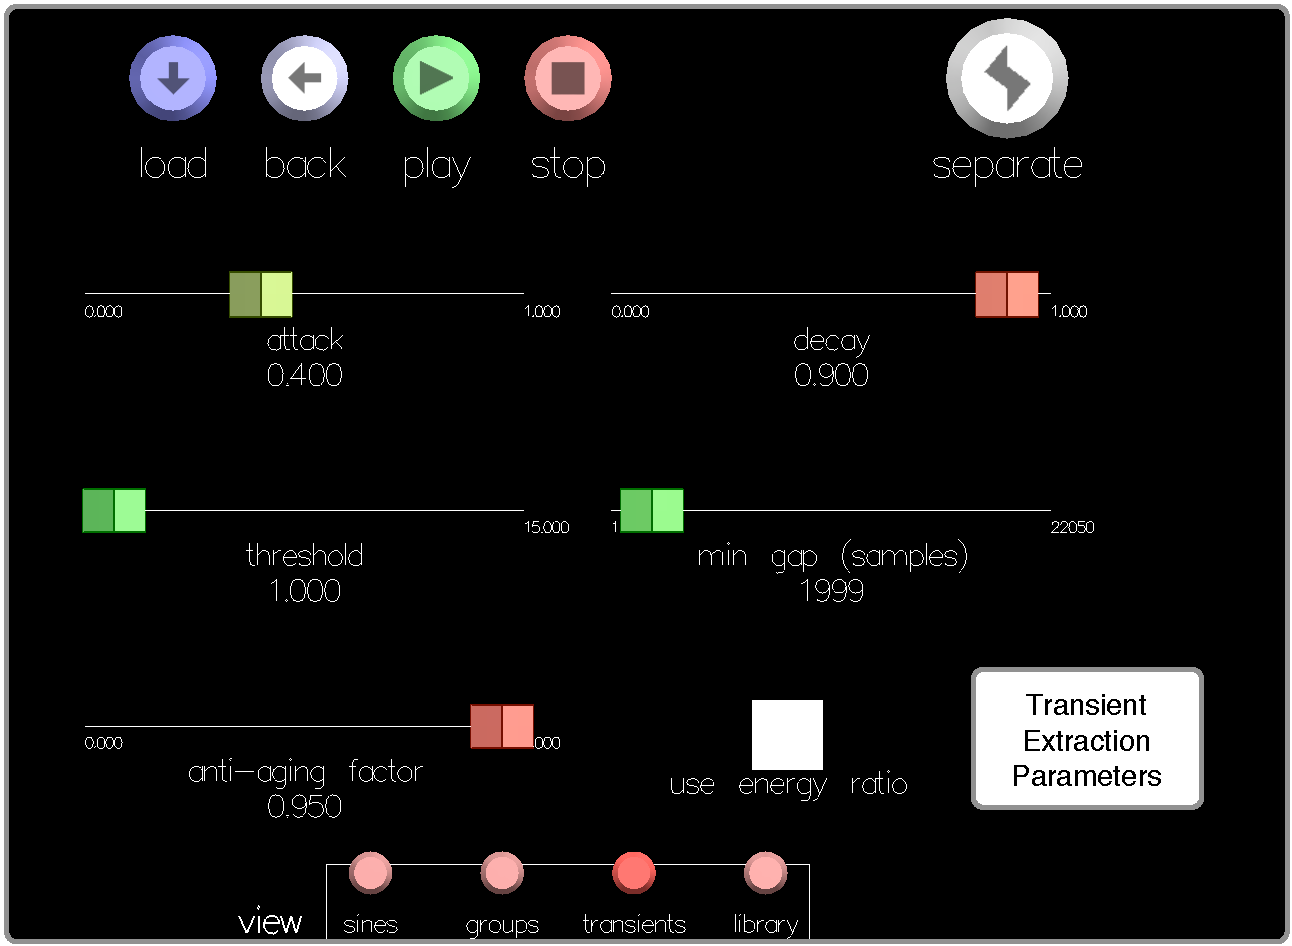
\includegraphics[width=.48\columnwidth]{ui_sliders3.pdf}}
    \caption{Sliders for sinusoidal analysis.} 
    \label{fig:ui_sines}
  \end{center}
\end{figure}

Undiscarded tracks are optionally
grouped~\cite{Ellis94,Melih00} by harmonicity, common amplitude
and frequency modulation, and common onset/offset (Figure \ref{fig:ui_sliders_group}), to form deterministic
events, which are essentially collections of related sinusoidal tracks.
If the grouping option is not selected, each track is interpreted as a
separate deterministic event. After this separation, the sinusoidal tracks found are marked on the spectrogram display. Each deterministic event can be individually played and saved as a template for use in the synthesis phase. 

\begin{figure}[h]
  \begin{center}
%    \framebox[7cm]{\rule[-5mm]{0cm}{5cm} }
    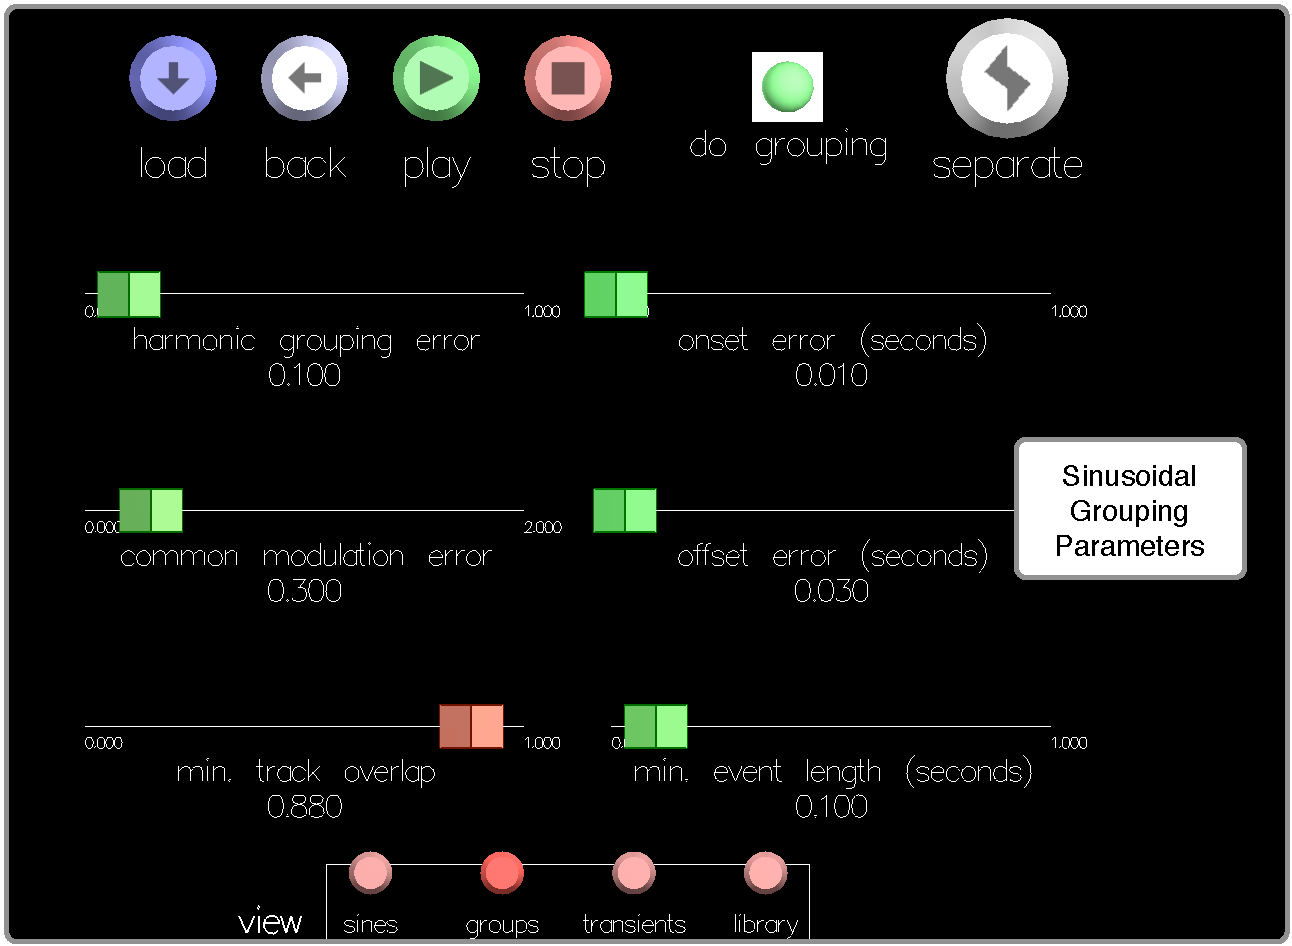
\includegraphics[width=.95\columnwidth]{ui_sliders2.pdf}
    \caption{Sliders for grouping sinusoidal tracks.} 
    \label{fig:ui_sliders_group}
  \end{center}
\end{figure}

\textit{Transient events} or brief noisy foreground events are usually
detected in the time-domain by observing changes in signal energy over
time~\shortcite{Verma98,Bello05}. TAPESTREA analyzes the recorded
sound using a non-linear one-pole envelope follower filter with a sharp
attack and slow decay and finds points where the derivative of the
envelope is above a threshold. These points mark sudden increases in
energy and are interpreted as transient onsets. A transient event is
considered to last for up to half a second from its onset; its exact
length can be controlled within that range. This length as well as the attack and
decay for the envelope follower filter, and the energy threshold for what
consitutes a transient can all be modified in real-time via sliders (Figure \ref{fig:ui_sliders_tran}). Detected transients can be
individually replayed and saved as templates. 

\begin{figure}[h]
  \begin{center}
%    \framebox[7cm]{\rule[-5mm]{0cm}{5cm} }
    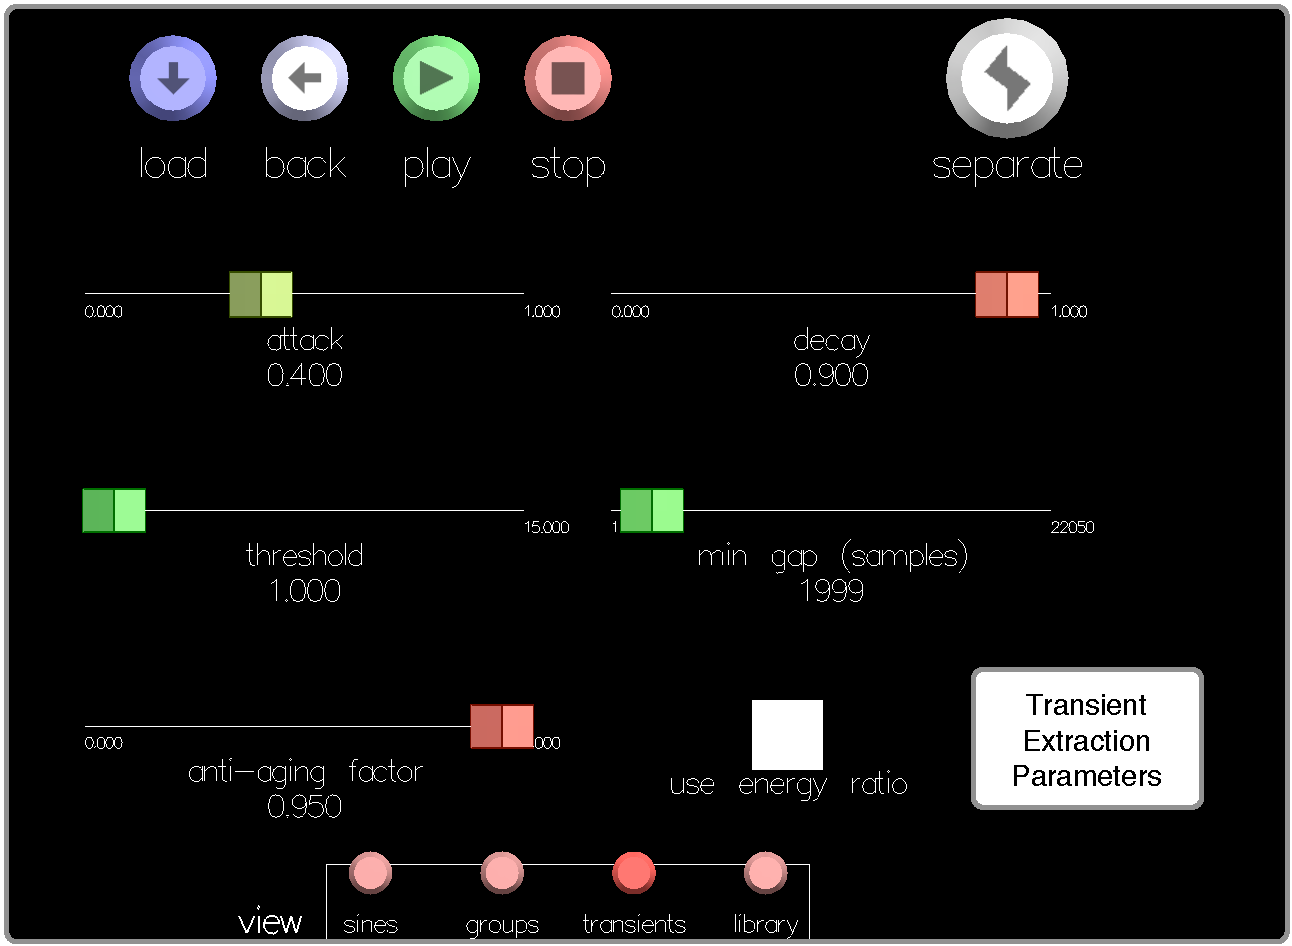
\includegraphics[width=.95\columnwidth]{ui_sliders3.pdf}
    \caption{Transient analysis sliders.} 
    \label{fig:ui_sliders_tran}
  \end{center}
\end{figure}

The \textit{stochastic background} represents parts of the recording that
constitute background noise, and is obtained by removing the detected
deterministic and transient events from the original sound. Deterministic
events are removed by eliminating the peaks of each sinusoidal track from
the corresponding spectral frames. To eliminate a peak, the magnitudes of
the bins beneath the peak are smoothed down, while the phases in these bins
are randomized (Figure \ref{fig:ui_separate}). Transient events, in turn, are removed in the time-domain by applying wavelet tree learning~\shortcite{Dubnov02} to generate a sound clip
that resembles nearby transient-free segments of the original recording.
This synthesized ``clean'' background replaces the samples containing the
transient event to be removed. Once separated, the stochastic background can be saved, played, or loaded into the interface for further analysis. 

\begin{figure}[h]
  \begin{center}
%    \framebox[7cm]{\rule[-5mm]{0cm}{5cm} }
    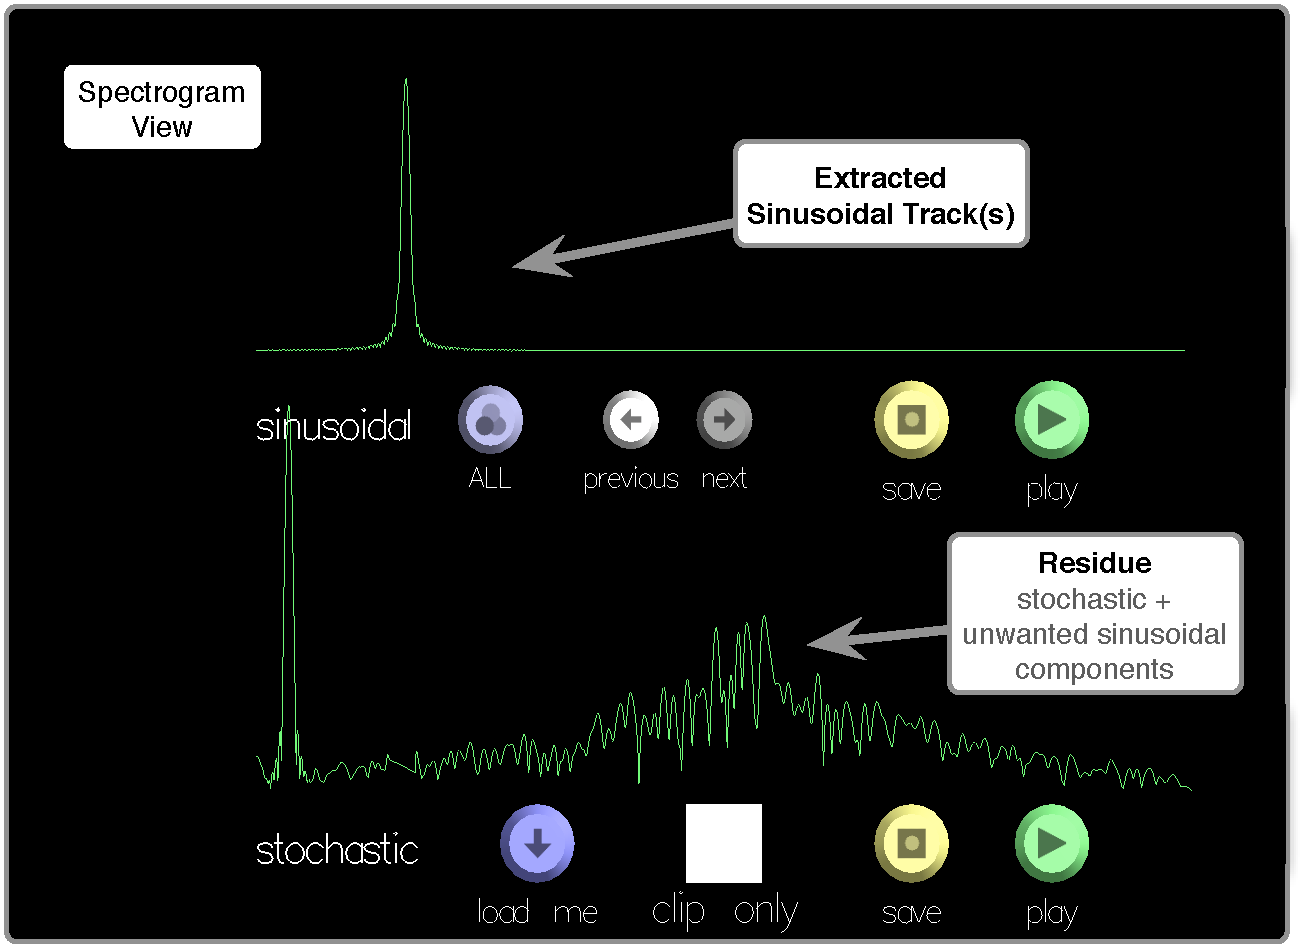
\includegraphics[width=.95\columnwidth]{ui_separate.pdf}
    \caption{Spectrum of separated sinusoidal peaks (top) and stochastic residue (bottom).} 
    \label{fig:ui_separate}
  \end{center}
\end{figure}

Separating a sound into components in this way has several
advantages. The distinction between foreground and background
components is semantically clear to humans, who can
therefore work within the framework with a concrete understanding
of what each component represents. The different
types of components are also stored and processed differently
according to their defining characteristics, thus allowing
flexible transformations on individual components. Each
transformed component can be saved as a template and later
reloaded, reused, copied, further transformed, or otherwise
treated as a single object. In addition, the act of separating a
sound into smaller sounds makes it possible to ``compose'' a
variety of pieces by combining these constituents in diverse
ways.

\section{Synthesis Phase}

\begin{figure}[h]
  \begin{center}
%    \framebox[7cm]{\rule[-5mm]{0cm}{5cm} }
    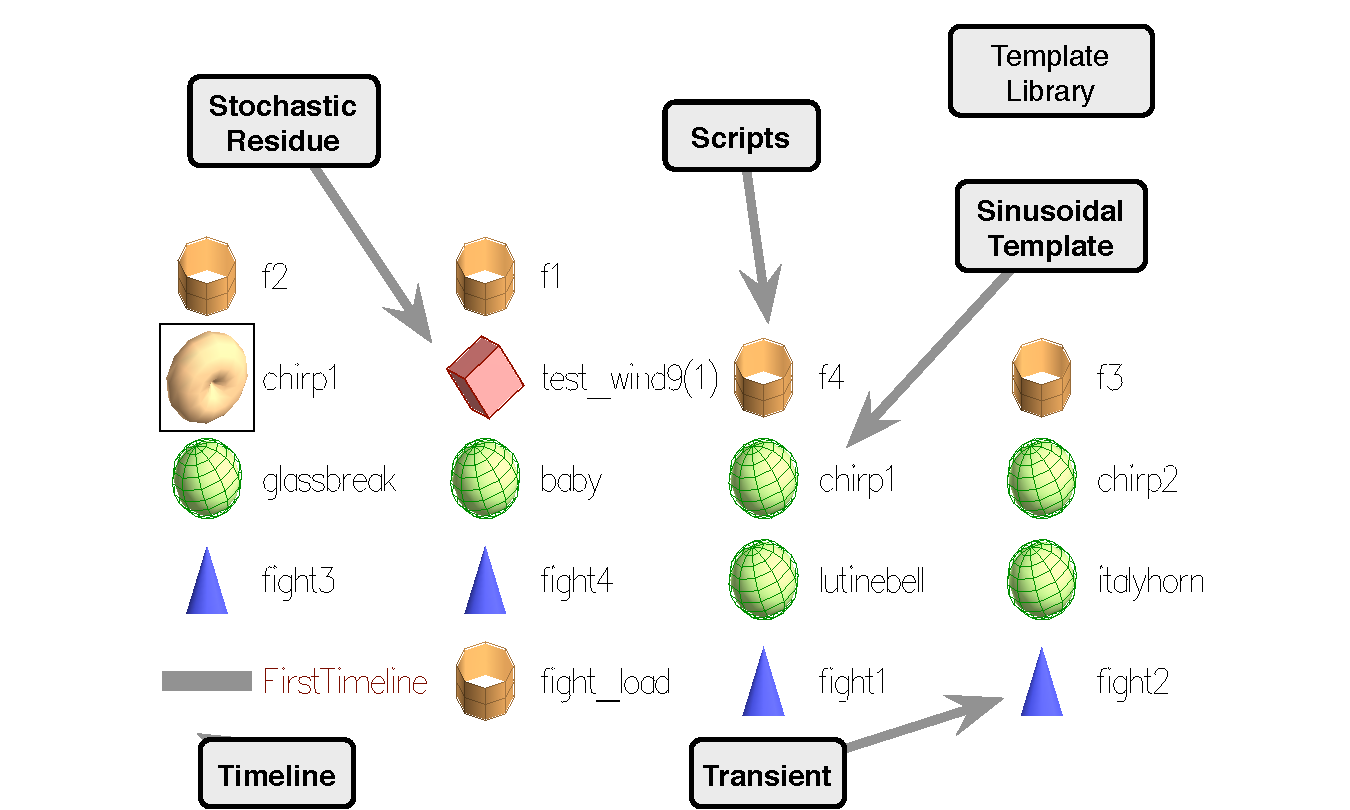
\includegraphics[width=.95\columnwidth]{ui_library.pdf}
    \caption{Library of saved templates.} 
    \label{fig:ui_library}
  \end{center}
\end{figure}

Once the components of a sound have been separated and saved as
templates, TAPESTREA allows each template to be transformed and
synthesized individually. The synthesis interface (Figure \ref{fig:ui_synthesis}) provides access to the current library of saved
templates, displayed as objects based on their type (Figure \ref{fig:ui_library}). Templates saved to file from prior sittings can be loaded into the library, too. Selecting
any template in the library displays a set of parameters suited to the
template type, exerting control over its transformation and synthesis. 
A selected template can be synthesized to generate
sound at any time, including while its transformation parameters are
being modified. At this point, TAPESTREA also offers
additional synthesis templates to control the placement or distribution
of basic components in a composition. The transformation and synthesis
options for the different template types are as follows:

\begin{figure}[h]
  \begin{center}
%    \framebox[7cm]{\rule[-5mm]{0cm}{5cm} }
    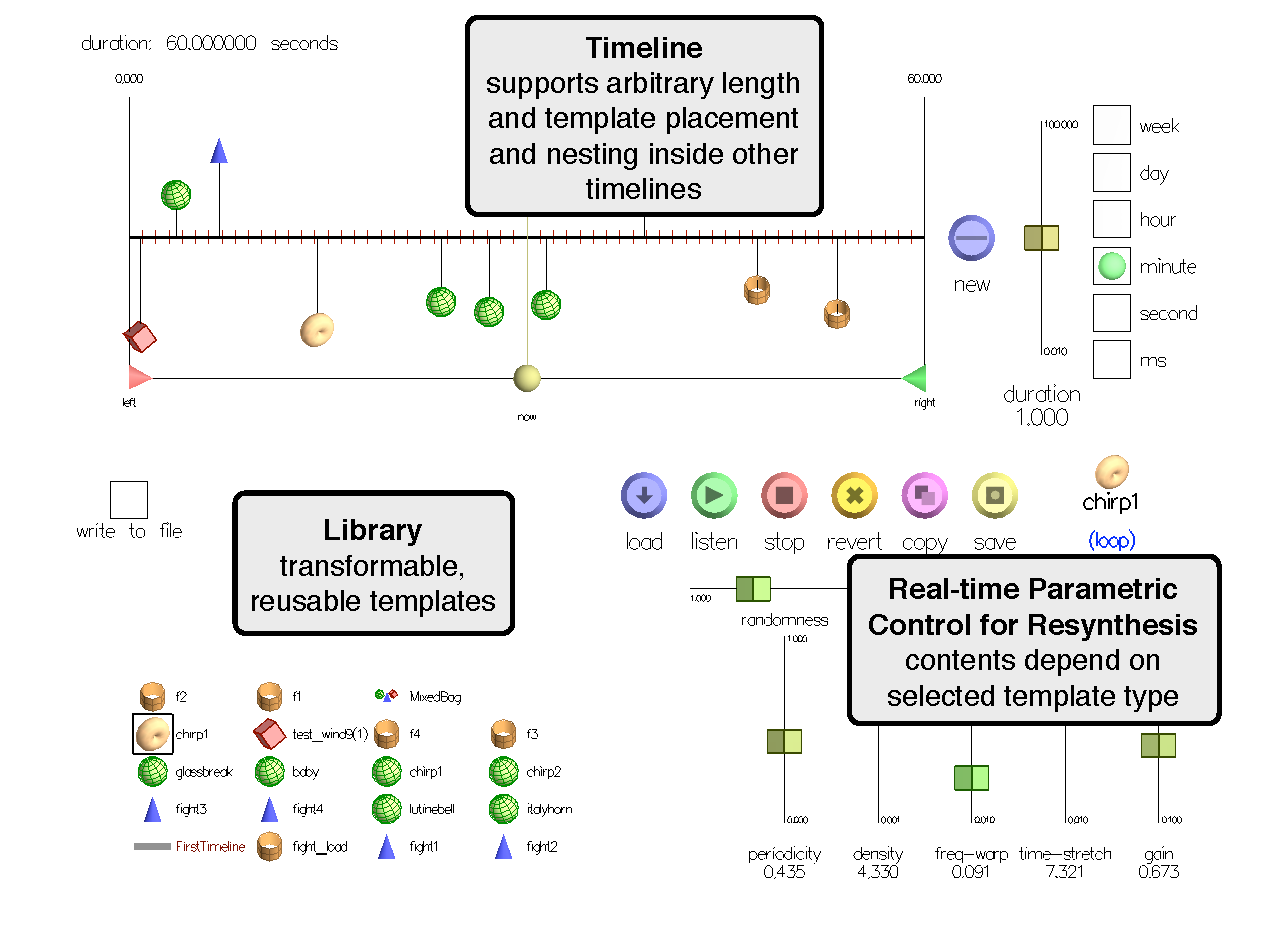
\includegraphics[width=.95\columnwidth]{ui_synthesis.pdf}
    \caption{Screenshot of transformation + synthesis interface.} 
    \label{fig:ui_synthesis}
  \end{center}
\end{figure}

\subsection{Deterministic Events} 

Deterministic events are synthesized from their tracks using sinusoidal
re-synthesis. Frequency and magnitude between consecutive frames in a
track are linearly interpolated, and time-domain samples are computed
from this information. 

The track representation allows considerable flexibility in applying
frequency and time transformations on a deterministic event. The event's
frequency (related to its pitch) can be linearly scaled before computing
the time-domain samples, simply by multiplying the frequency at each
point on its tracks by a specified factor. Similarly, the event can be
stretched or shrunk in time by scaling the time values in the
time-to-frequency trajectories of its tracks. This technique works for
almost any frequency or time scaling factor without producing artifacts.
Frequency and time transformations can take place in real-time in
TAPESTREA, thus allowing an event to be stretched, shrunk or pitch
shifted even as it is being synthesized.

\subsection{Transient Events} 

Since transient events are brief by definition, TAPESTREA stores them
directly as time-domain audio frames. Synthesizing a transient event
without any transformations, therefore, involves playing back the
samples in the audio frame. 

In addition, TAPESTREA allows time-stretching and pitch-shifting in
transient events as well. This is implemented using a phase
vocoder~\cite{Dolson86}, which limits the scaling factors to a range smaller
and perhaps more reasonable than what is available for deterministic events,
yet large enough to create noticeable effects.

Transient events by nature can also act as ``grains'' for traditional
granular synthesis~\cite{Truax88,Truax90,Roads02}. The
frequency and time transformation tools for transients, along with the
additional synthesis templates described in Sections 4.4 to 4.6, can
thus provide an interactive ``granular synthesis'' interface.

\subsection{Stochastic Background}

The internal representation of a \textit{stochastic background} template
begins with a link to a sound file containing the related background
component extracted in the analysis phase. However, merely looping
through this sound file or randomly mixing segments of it does not
produce a satisfactory background sound. Instead, our goal here is to
generate ongoing background that sounds controllably similar to the
original extracted stochastic background. 

Therefore, the stochastic background is synthesized from the saved sound
file using an extension of the wavelet tree learning
algorithm~\shortcite{Dubnov02}. In the original algorithm, the saved
background sound is decomposed into a wavelet tree where each node
represents a wavelet coefficient, with depth corresponding to resolution.
The wavelet coefficients are computed using the Daubechies wavelet with 5
vanishing moments. A new wavelet tree is then built, with each node selected
based on the similarity of its ancestors and its first \textit{k} predecessors
(nodes at the same depth but associated with earlier time samples) to
corresponding sequences of nodes in the original tree. The learning
algorithm also takes into account the amount of randomness desired. Finally,
the new wavelet tree undergoes an inverse wavelet transform to provide the
synthesized time-domains samples. This learning technique works best with
the separated stochastic background as input, since the sinusoidal events it
would otherwise chop up have been removed.

TAPESTREA uses a modified and optimized version of the algorithm, which
follows the same basic step except in some details. For instance, the
modified algorithm includes the option of incorporating randomness into
the first level of learning, and also considers \textit{k} as dependent on
the depth of a node rather than being constant. More importantly, it
optionally avoids learning the coefficients at the highest resolutions.
These resolutions roughly correspond to high frequencies, and randomness
at these levels does not significantly alter the results, while the
learning involved in attaining that randomness takes the most time.
Optionally stopping the learning at a lower level thus optimizes the
algorithm and allows it to run in real-time. 

Further, TAPESTREA offers interactive control over the learning
parameters in the form of ``randomness'' and ``similarity'' parameters. The
size of a sound segment to be analyzed as one unit can also be
controlled, and results in a ``smooth'' synthesized background for larger
sizes versus a more ``chunky'' background for smaller sizes. Creatively
manipulating these parameters can, in fact, yield interesting (and
weird) musical compositions generated through ``stochastic background''
alone.

\subsection{Event Loops}

\begin{figure}[h]
  \begin{center}
%    \framebox[7cm]{\rule[-5mm]{0cm}{5cm} }
    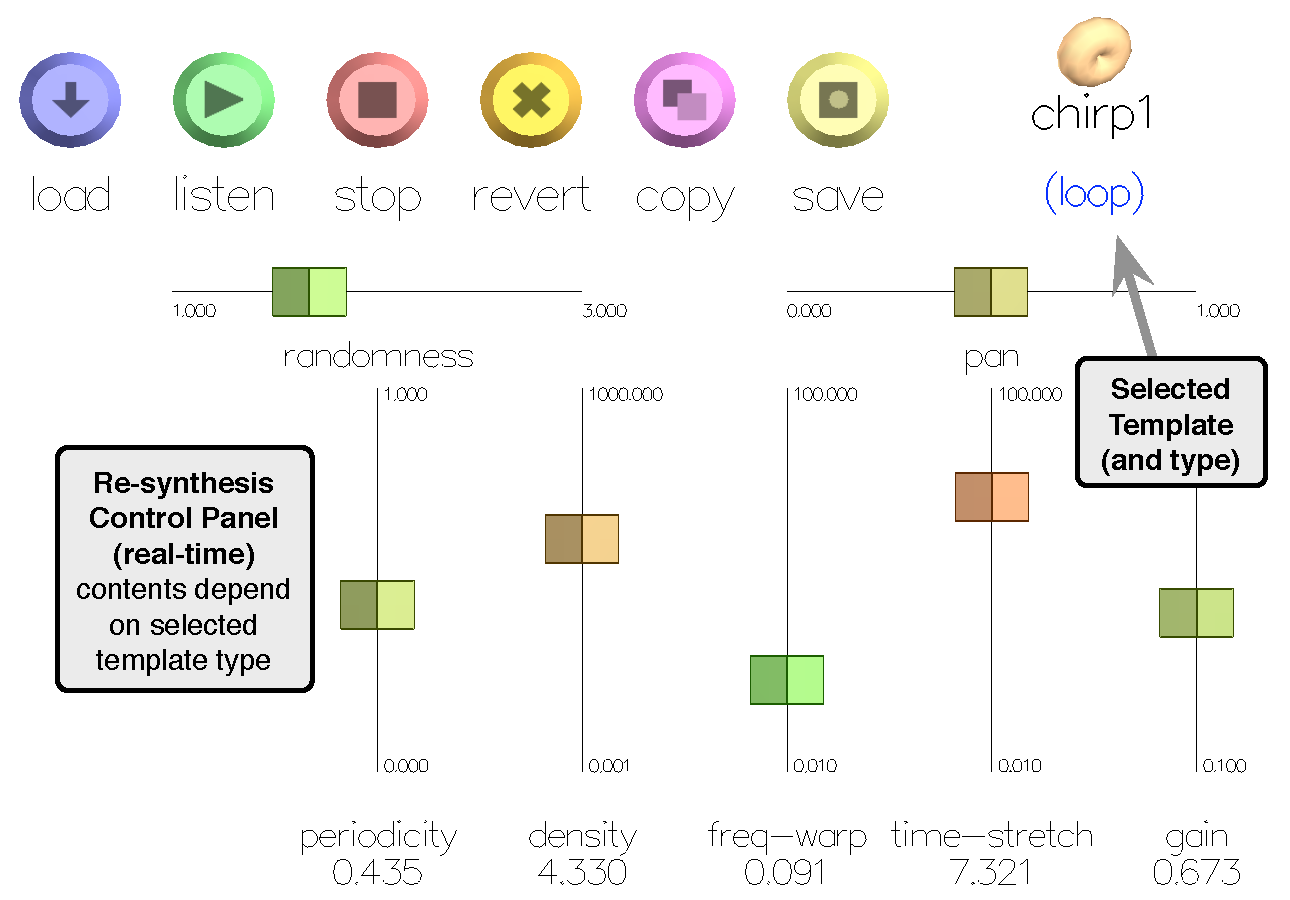
\includegraphics[width=.95\columnwidth]{ui_params.pdf}
    \caption{Sliders for controlling an event loop.} 
    \label{fig:ui_loop_params}
  \end{center}
\end{figure}

Event loops (Figure \ref{fig:ui_loop_params}) are synthesis templates designed to facilitate the
parametric repetition of a single event. Any deterministic or transient
event template can be formed into a loop. When the loop is played,
instances of the associated event are synthesized at the specified
density and periodicity, and within a specified range of random
transformations. These parameters can be modified while the loop is
playing, to let the synthesized sound change gradually. 

The density refers to how many times the event is repeated per second,
and could be on the order of 0.001 to 1000. At the higher densities, and
especially for transient events, the synthesized sound is often
perceived as continuous, thus resembling granular synthesis. 

The periodicity, ranging from 0 to 1, denotes how periodic the
repetition is, with a periodicity of 1 meaning that the event is
repeated at fixed time intervals. The interval between consecutive
occurrences of an event is generally determined by feeding the desired
periodicity and density into a Gaussian random number generator. It is
straightforward to replace this generator with one that follows a
Poisson or other user-specified probability distribution. 

In addition to the parameters for specifying the temporal placement of
events, TAPESTREA allows each instance of the recurring event to be
randomly transformed within a range. The range is determined by selected
average frequency- and time-scale factors, and a randomness factor that
dictates how far an individual transformation may vary from the average.
Individual transformation parameters are uniformly selected from within
this range. Apart from frequency and time scaling, the gain and pan of
event instances can also randomly vary in the same way.

\subsection{Timelines}

While a loop parametrically controls the repetition of a single event,
with some amount of randomization, a timeline allows a template to be
explicitly placed in time, in relation to other templates. Any number of
existing templates can be added to a timeline, as well as deleted from
it or re-positioned within it once they have been added. 

A template's location on the timeline indicates its onset time with
respect to when the timeline starts playing. When a timeline is played,
each template on it is synthesized at the appropriate onset time, and is
played for its duration or till the end of the timeline is reached. The
duration of the entire timeline can be on the order of milliseconds to
weeks, and may be modified after the timeline's creation. 

TAPESTREA also allows the placement of timelines within timelines (or
even within themselves). This allows for template placement to be
controlled at multiple time-scales or levels, making for a
``multiresolution synthesis.''

\subsection{Mixed Bags}

Another template for synthesis purposes is the mixed bag (Figure \ref{fig:ui_mixedbag_params}), which is
designed to control the relative densities of multiple, possibly
repeating, templates. Like a timeline, a mixed bag can contain any
number of templates, but these templates are randomly placed in time and
transformed, as in loops. The goal is to facilitate the synthesis of a
composition with many repeating components, without specifying precisely
when each event occurs. The real-time parameters for controlling this
also enable the tone of a piece to change over time while using the same
set of components, simply by synthesizing these components differently. 

\begin{figure}[h]
  \begin{center}
%    \framebox[7cm]{\rule[-5mm]{0cm}{5cm} }
    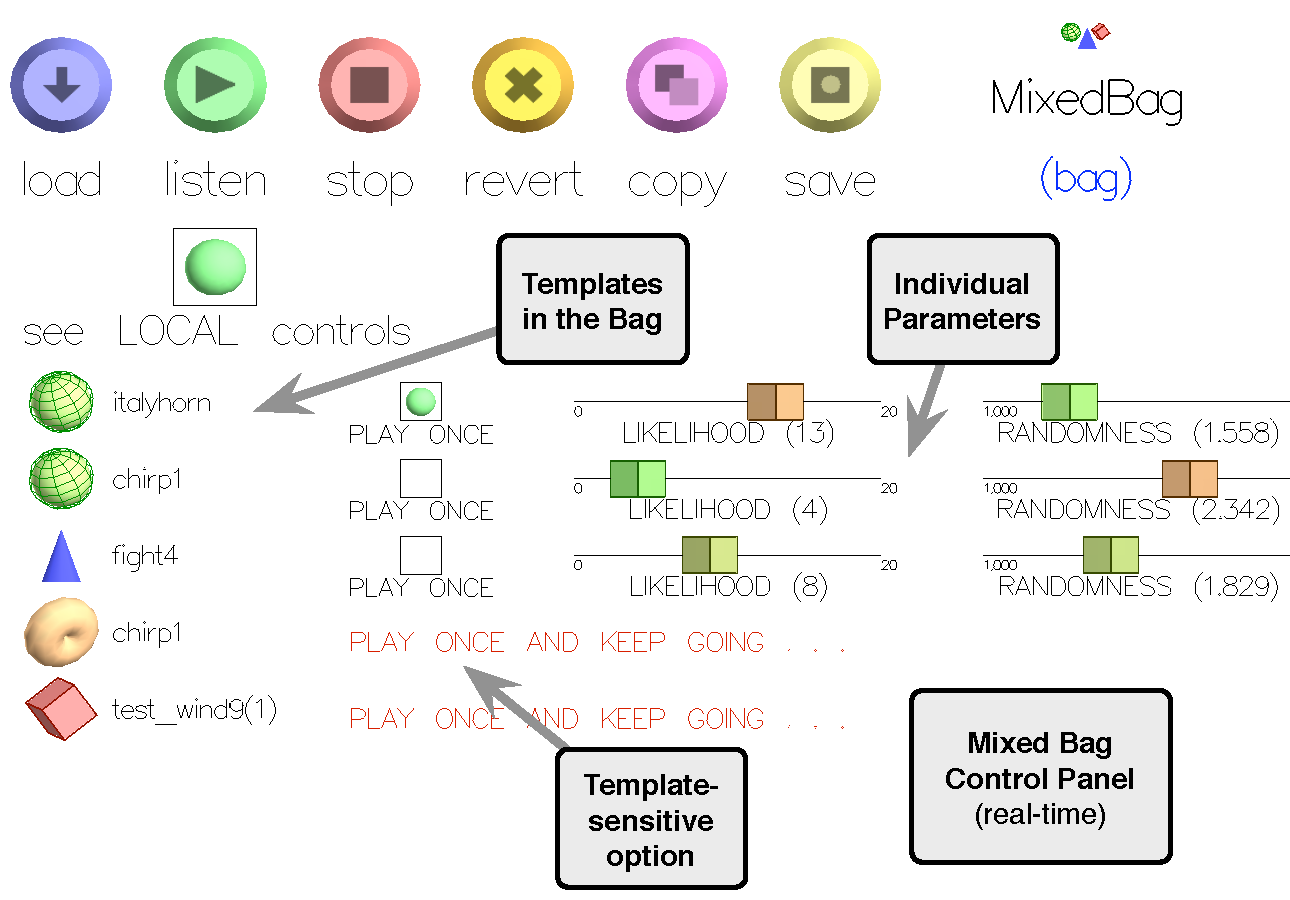
\includegraphics[width=.95\columnwidth]{ui_mixedbag.pdf}
    \caption{Sliders for controlling items in a mixed bag.} 
    \label{fig:ui_mixedbag_params}
  \end{center}
\end{figure}

When a template is added to a mixed bag, it can be set to play either
once or repeatedly. It also has a ``likelihood'' parameter, which
determines the probability of that template's being played in preference
over any of the other templates in the bag. Finally, it has a
``randomness'' parameter, which controls the range for random
transformations on that template, analogous to the randomness control in
event loops.

Beyond these individual template parameters, each mixed bag has overall
periodicity and density settings, which control the temporal
distribution of repeating templates in the same way that an event loop
does. However, while an event loop plays instances of a single event, a
mixed bag randomly selects a repeating template from its list whenever
it is time to synthesize a new instance. Templates with higher
likelihood settings are more likely to be selected for synthesis. 

One way to think of a mixed bag is as a physical bag of marbles. The
overall periodicity and density parameters determine how often someone
dips his hand in the bag and pulls out a marble, or a template to be
synthesized. The likelihood setting of a template or marble controls how
likely it is for the hand to pull out that particular marble. A
repeating marble is tossed back into the bag as soon as it is
drawn and observed (played).

\subsection{Pitch and Time Quantizations}

While sliders control the synthesis parameters in a continuous way, more customized musical control can be exerted by quantizing pitches and times to user-specified values. Pitch and time tables can be loaded on-the-fly for each template. 

The frequency scaling factor of a template is quantized to the the nearest entry in its pitch table, if it has one. This directly influences the frequency at which a deterministic or transient event is synthesized. For event loops and mixed bags, it controls the possible frequency scaling during random transformations on the underlying events. The frequencies of individual templates on a timeline are scaled, in the order in which they are played, by successive entries on the timeline's pitch table. This allows a user-defined musical scale to be applied to most templates. 

Rhythm can be similarly specified by quantizing time to the nearest entry in a time table. In event loops and mixed bags, this quantizes the event density parameter as well as the intervals between consecutive events. On timelines, templates are positioned only at time points corresponding to table entries, if a table exists. Thus, templates can can start synthesizing at particular beats. 

\subsection{Score Language}

The manipulations described so far primarily occur through a
visual interface. Even finer control over the synthesis can be obtained
through the use of a score language. The audio programming language
ChucK~\cite{Wang03} is used here both for specifying precise
parameter values and for controlling exactly how these values change
over time. 

* Paragraph or two about ChucK?  GE WRITE THIS.

* Paragraph on key (i.e. implemented) features.  AND THIS. [A score can be loaded as a template and played at any time.]

\subsection{Other Controls}

Beyond the synthesis parameters mentioned so far, TAP-ESTREA offers some
generic synthesis and playback controls. The gain and stereo panning of
individual templates can be controlled individually, and can be randomly
set for templates in event loops and mixed bags. A reverb effect adapted
from STK~\cite{Cook99} can also be added to the final synthesized sound.

The synthesis interface also provides a number of ways to instantiate new templates. Any
existing template can be copied, while deterministic and transient event
templates can also be saved as event loops. New timelines and mixed bags
can be freely created, and existing templates can be dragged onto or off
these as needed. Templates can also be deleted from the library,
provided they are not being used in a timeline or a mixed bag. Finally,
while sound is generally synthesized in real-time, TAPESTREA offers the
option of writing the synthesized sound to file.

\section{Discussion}


\section{Conclusion}

There is no end to the 

%\subsection{A Subsection}

%The Latex source, \textsf{icmc2006template.tex}, contains comments
%explaining how you should use Latex so as to conform to the paper
%format guidelines.

% \paragraph conforms to the guidelines; \subsubheading doesn't.
% I'll grant you that \paragraph is logically wrong, but it's easy.
%\paragraph{Third-order heading.}
%If you wish to use third-order headings, format them like this.  They
%start an unindented paragraph.

%Additional paragraphs are indented as usual.

%\subsection{References}

% We use chicago.(bst|sty), which supports (Author, year) cites and
% can be made to look _almost_ the way we wanted.  See chicago.sty
% for a list of all the flavors of citation you can do.
% \cite            (Laurel and Hardy 1932)
% \shortcite       (Laurel et al. 1932)
% \citeN           Laurel and Hardy (1932)
% \shortciteN      Laurel et al. (1932)

%Bibliographical references appear in parentheses; there is an example
%at the end of this sentence~\cite{canon}.  References with up to
%three authors include all the authors \cite{fugue}, but references
%with more than three authors use ``et al.''
% that is, you use \shortcite
%\shortcite{ircam-mw}.\footnote{Here is a footnote I hope you enjoy it.}
% (My naive attempt at hacking chicago.bst to do it had the side effect
% of leaving no space between the author and the "et".  We decided the
% italics were less than utterly indispensable.  If you know how to
% get them, though, drop me a note at eli@cs.cmu.edu.)

%A reference is not a subject or object. When you want to use the
%referenced work as part of a sentence, use the author or authors and
%use the year only for the reference, as in the following sentence:
% \citeN is "cite as noun"
%\citeN{mathews} includes a manual for Music V\@.  
% or if you want to, you can say
% Mathews~\citeyear{mathews} includes a manual for Music V\@.  

%Just for variety, this is a reference to an ICMC
%paper~\cite{superscalar}.

%\subsection{Figures and Captions}

%Place all figures in-line with the text.  Please include an
%explanatory caption for each.

%\begin{figure}[htbp]
%  \begin{center}

%    \framebox[7cm]{\rule[-5mm]{0cm}{5cm} }

%    \caption{This figure intentionally left blank.} 
%    \label{fig:emptybox}
%  \end{center}
%\end{figure}

%\section{Copyright Notices}

%You may wish to add a copyright notice to the bottom of the first
%column of your paper.  All copyrights remain with the authors.
%Authors will be asked to sign a form that gives ICMA, ICMC, and IEEE
%rights to sell the ICMC proceedings.  Typically, ICMC papers carry no
%explicit copyright notice.

\bibliographystyle{chicago}
\small{
\bibliography{taps_icmc2006}
}

\end{document}
